% Existing bitmap is preserved byte-for-byte; viewport only changes presentation.
% Raster is 2400 x 1240 at approximately 200 dpi. Crops retain both rows.
\begin{figure*}[tp]
\centering
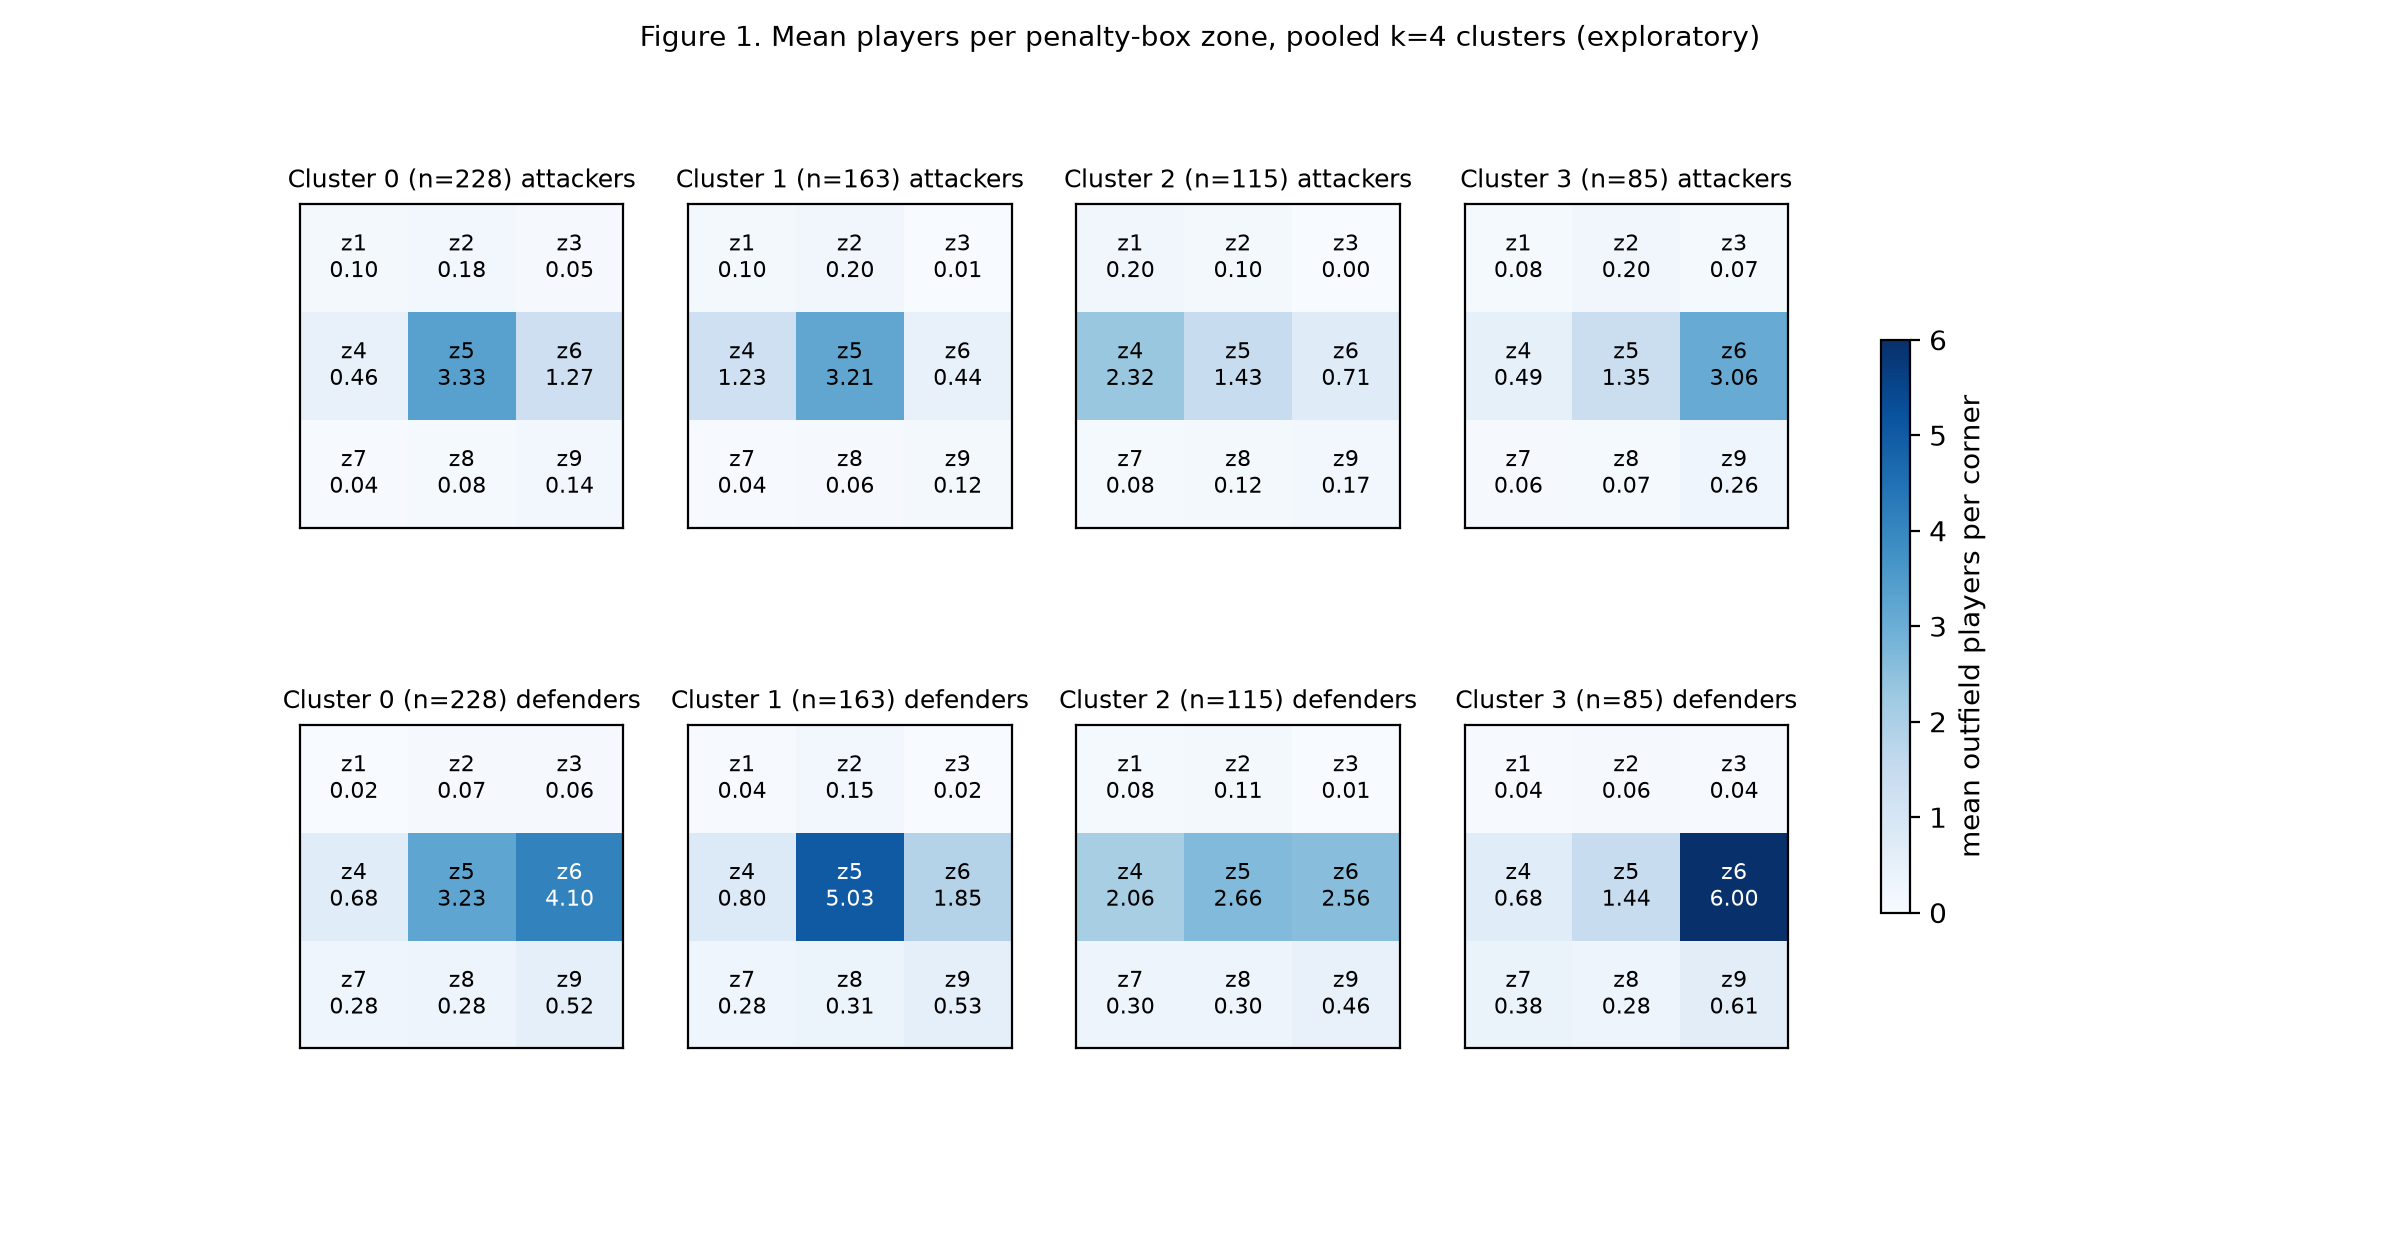
\includegraphics[width=0.68\textwidth,viewport=100.8 64.8 372.6 390.6,clip]{figures/cluster-zone-means.png}
\caption{Mean attacking (top) and defending (bottom) outfield occupancy by penalty-box zone for shared clusters 0 (228 corners) and 1 (163). Columns increase in x toward the goal (right); rows increase in y down the image. Zones z3/z6/z9 are goal-nearest; z7--z9 are in the high-y, normalized corner-side band. These are schematic cells, not trajectories. The common blue scale is 0--6 mean observed players, shown with the companion panel in Figure~\ref{fig:zones23}. Keepers and the taker are excluded. Source: \href{https://github.com/ImpalaOcean/corner-scouting/blob/77af6f910935b6b12232b3e60183210c7f175e56/docs/spatial-results/reports/k4_cov0.5.json}{saved primary setup report}, verified to displayed two-decimal precision; evidence X3/F2. The full-tournament pooled fit is retrospective and exploratory, with incomplete, delivery-selective visibility.}
\Description{Two enlarged cluster panels, each with attackers above defenders in a numbered three-by-three grid. Cluster 0 has 3.33 attackers in zone 5 and 4.10 defenders in zone 6; cluster 1 has 3.21 attackers and 5.03 defenders in zone 5. These are static observed means.}
\label{fig:zones01}
\end{figure*}

\begin{figure*}[tp]
\centering
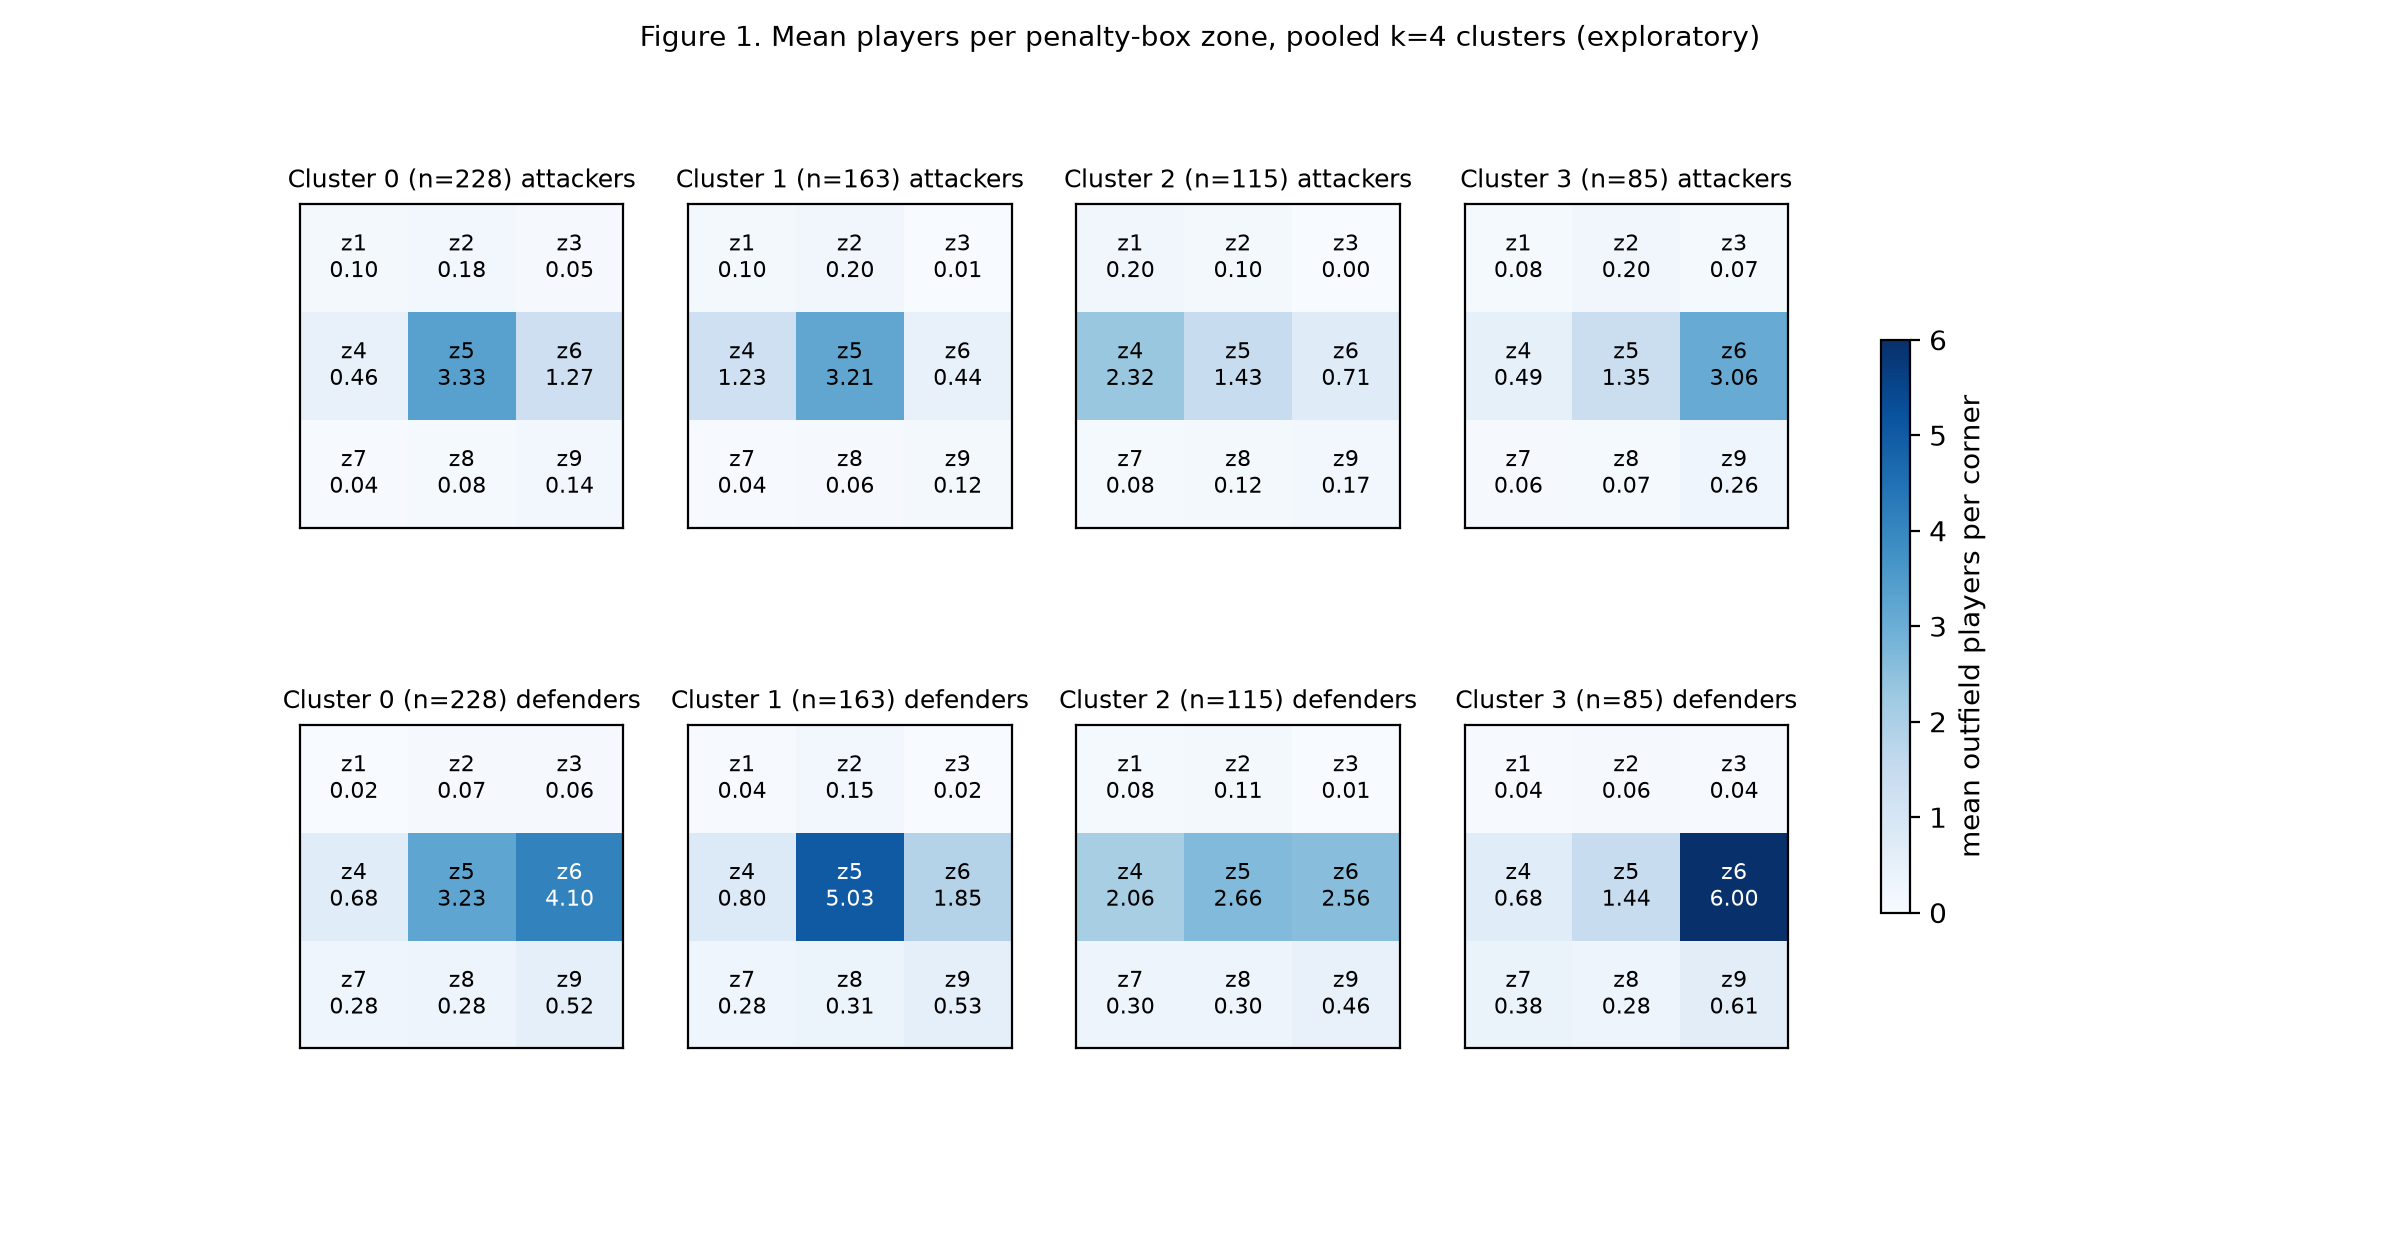
\includegraphics[width=0.75\textwidth,viewport=374.4 64.8 721.8 390.6,clip]{figures/cluster-zone-means.png}
\caption{Companion panels for shared clusters 2 (115 corners) and 3 (85), preserving the same existing image and common 0--6 colour scale. Top/bottom grids show mean observed attacking/defending outfield occupancy. As in the companion panel, the goal lies right and the normalized high-y corner is beyond the bottom edge of each grid. Together Figures~\ref{fig:zones01}--\ref{fig:zones23} display all four clusters, not selected teams or successful routines. Source: \href{https://github.com/ImpalaOcean/corner-scouting/blob/77af6f910935b6b12232b3e60183210c7f175e56/docs/spatial-results/reports/k4_cov0.5.json}{saved primary setup report}; evidence X3/F2. Cluster 3 has 6.00 mean defenders in zone 6; this is not a marking-scheme label or tactical-quality score. Partial visibility and team-level small samples limit interpretation. These retrospective centres must not enter a prematch dossier without a separate past-only fit.}
\Description{Clusters 2 and 3 are shown as attacker and defender zone grids beside a shared colour bar. Cluster 2 has 2.32 attackers in zone 4; cluster 3 has 3.06 attackers and 6.00 defenders in zone 6. Values summarize delivery-time snapshots, not movement.}
\label{fig:zones23}
\end{figure*}
